\chapter{General Functions of a Complex Variable}
If you want to study some space, study how function behaves there. While considering $\Bbb{C}$ as a vector space $\Bbb{R}^2$ with some more structure, we can see how a general function may look in a complex plane. Let's say, $f:\Bbb{C}\rightarrow\Bbb{C}$ where $z\mapsto w=f(z)$. Then if we want to plot the input-output pair, $(z,f(z))$ isn't we need $4$ dimensions, $(2\dim,2\dim)$? Don't worry, there are $5$ different ways to solve this problem and visualize the complex functions:
\begin{itemize}
    \item Domain Coloring 
    \item $3D$ Plots
    \item Vector Fields
    \item $z-w$ Planes
    \item Riemann Sphere
\end{itemize}

In the Domain Coloring method, we associate the output with a color representing the complex number $f(z)$. Where, 
\begin{align*}
    \text{Hue}&\leftrightarrow\text{Argument}\\
    \text{Lightness}&\leftrightarrow\text{Modulus}
\end{align*}

In the $3D$ Plots method, we sacrifice one real variable from $(z,f(z))=(x,y,u,v)$ and associate the missing variable with a color representing the missing complex number $v$. 
$$\text{Missing }v\leftrightarrow\text{color}$$
For more details have a look at \url{https://www.youtube.com/watch?v=NtoIXhUgqSk}. 

\begin{defn}
A multi-valued function $f$ on $E\subset\mathbb C$ assigns a set of complex values to each $z\in E$, i.e. $f(z)$ is a set of complex numbers.
\end{defn}

\begin{defn}
    A branch of a multi-valued function $f$ on $E\subset\mathbb C$ is a function that assigns to each $z\in E$ one value from $f(z)$. 
\end{defn}
\section{Sometimes, mapping is not what you want so!}
For any function, $f(z):D\subseteq\mathbb{C}\rightarrow\mathbb{C}$ we can understand the function examining the outputs. Like, if we consider the inputs $z=x+iy$ then the output $w\in\mathbb{C}$ is also a complex number and we can say the complex function $f(z)$ is a pair of real functions. 
\begin{align*}
    w&=f(z)\\
    &=f(x+iy)\\
    &=u+iv\\
    &=u(x,y)+iv(x,y)
\end{align*}
That means rather than understanding the complex function $f(z)$, we can understand the real functions $u(x,y)$ and $v(x,y)$. Similarly, in polar form $z=re^{i\theta}$ we get, 
\begin{align*}
    w&=f(z)\\
    &=f(re^{i\theta})\\
    &=u+iv\\
    &=u(r,\theta)+iv(r,\theta)
\end{align*}
Which one we need to use depends on the function you have given. Okay, now we will see how $\exp(z)$, $\log(z)$ and $z^2$ function work. 
\subsection{Complex Exponential}
The exponential function, $$\exp:\mathbb{C}\rightarrow\mathbb{C}-\{0\}$$
is defined to be $$\exp(z)=\exp(x+iy)=e^xe^{iy}$$
Wait, isn't $e^{iy}=\cos(y)+i\sin(y)$? That means the output is a complex number which is naturally represented in a polar form whose modulus and argument are,
$$\mid\exp(x+iy)\mid=e^x\qquad\operatorname{arg}(\exp(x+iy))=y+2\pi\mathbb{Z}$$
\begin{tcolorbox}
Can you see why the exponential map is a homomorphism from the addition group $(\mathbb{C},+)$ to the multiplicative group $(\mathbb{C}-\{0\},\cdot)$? From this perspective, we can say,
$$\exp:(\mathbb{C}//2\pi\mathbb Z,+)\rightarrow(\mathbb{C}-\{0\},\cdot)$$
\end{tcolorbox}
How we can visualize this map? By using the $z-w$ plane. Let's see how this map acts for horizontal and vertical lines from $z$-plane to the $w$-plane. 
\begin{figure}[htbp]
    \centering
    % Left image
    \begin{subfigure}[b]{0.45\textwidth}
        \centering
        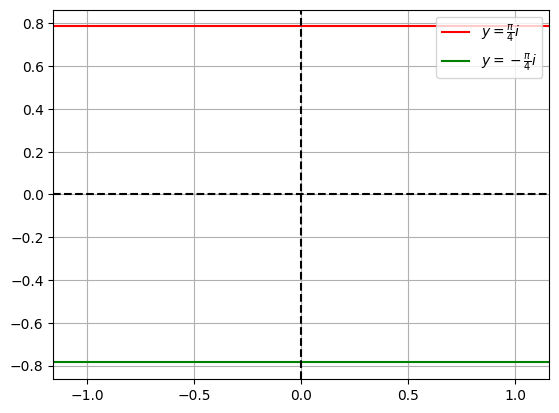
\includegraphics[width=\linewidth]{FIG_MAT215/exp z horizontal lines.png}
        \caption{$z = x \pm \frac{\pi}{4}i$}
        \label{fig:exp_inputs_h}
    \end{subfigure}
    \hfill
    % Right image
    \begin{subfigure}[b]{0.45\textwidth}
        \centering
        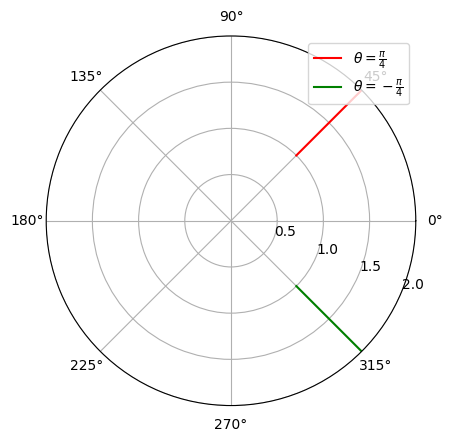
\includegraphics[width=\linewidth]{FIG_MAT215/exp z horizontal lines out.png}
        \caption{$r=e^x,\theta =\pm\frac{\pi}{4}$}
        \label{fig:exp_outputs_h}
    \end{subfigure}
    \caption{Input and Output under the Exponential Map for Horizontal Lines}
    \label{fig:exp_map_horizontal_lines}
\end{figure}
For $z=x+\frac{\pi}{4}i$ line (red), if we apply the complex exponent then we get,
\begin{align*}
    \exp{z}&=\exp\left({x+\frac{\pi}{4}i}\right)\\
    &= e^{x}e^{i\frac{\pi}{4}}
\end{align*}
Here, if we compare the final result with the complex polar form then we get $r=e^x$ and $\theta=\frac{\pi}{4}$. 
\begin{tcolorbox}
Wait, why not we use the rectangular form? Because $e^xe^{i\frac{\pi}{4}}=e^x\cos\frac{\pi}{4}+ie^x\sin\frac{\pi}{4}=u(x)+iv(x)$ is not a good choice for here, as it needs to be considered both real and imaginary part in term of a varying $x$ (as a function of $x$).    
\end{tcolorbox}
 That means our arguments are fixed but radii are changing. Hence, get the red line which is emitting from the origin with angle $\frac{\pi}{4}$. But here is a gotcha! why this ray is not coming from exactly the origin? Can you guess that? Similarly, we can have
\begin{align*}
    \exp{z}&=\exp\left({x-\frac{\pi}{4}i}\right)\\
    &= e^{x}e^{-i\frac{\pi}{4}}
\end{align*}
Okay, let's repeat the whole thing, but this time use the vertical lines in our input plane. 

\begin{figure}[htbp]
    \centering
    % Left image
    \begin{subfigure}[b]{0.45\textwidth}
        \centering
        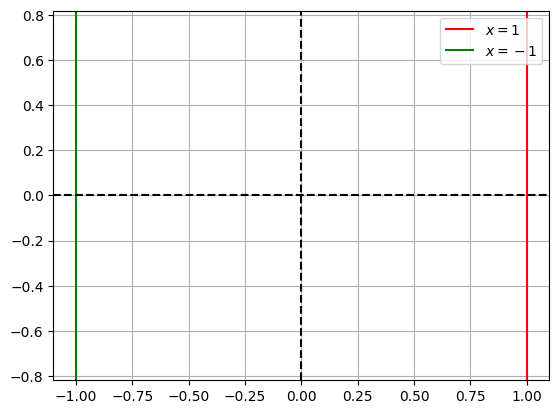
\includegraphics[width=\linewidth]{FIG_MAT215/exp z vertical lines.png}
        \caption{$z = \pm 1+iy$}
        \label{fig:exp_inputs_h}
    \end{subfigure}
    \hfill
    % Right image
    \begin{subfigure}[b]{0.45\textwidth}
        \centering
        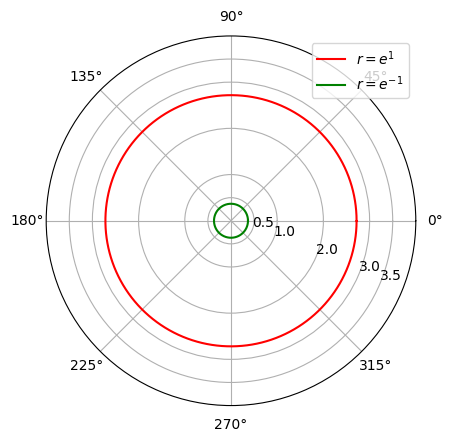
\includegraphics[width=\linewidth]{FIG_MAT215/exp z vertical lines out.png}
        \caption{$r=e^{\pm1}$}
        \label{fig:exp_outputs_h}
    \end{subfigure}
    \caption{Input and Output under the Exponential Map for Vertical Lines}
    \label{fig:exp_map_vertical_lines}
\end{figure}
For example, if we take the vertical line $z=1+iy$ whose $x$ coordinate is fixed and $y$ can vary then we have, 
\begin{align*}
    \exp{z}&=\exp\left(1+iy\right)\\
    &= e^{1}e^{iy}
\end{align*}
Again, if we compare the final result with the complex polar form then we get $r=e^1$ (fixed radius) and $\theta=y$ (which is changing). Hence, the end result is a circle with radius $r=e^1$ (red). I hope you can do the same for $z=-1+iy$. 
\begin{figure}[htbp]
    \centering
    % Left image
    \begin{subfigure}[b]{0.45\textwidth}
        \centering
        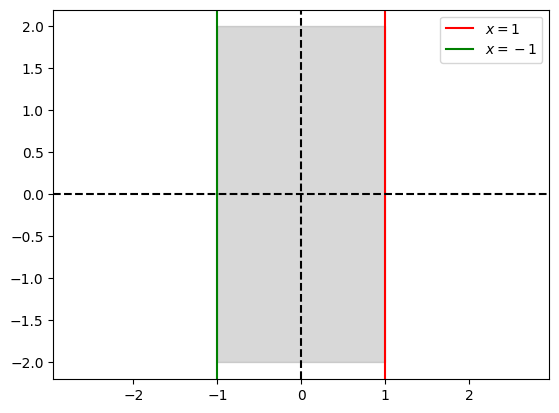
\includegraphics[width=\linewidth]{FIG_MAT215/exp z vertical strip.png}
        \caption{$z = \pm 1+iy$}
        \label{fig:exp_inputs_h}
    \end{subfigure}
    \hfill
    % Right image
    \begin{subfigure}[b]{0.45\textwidth}
        \centering
        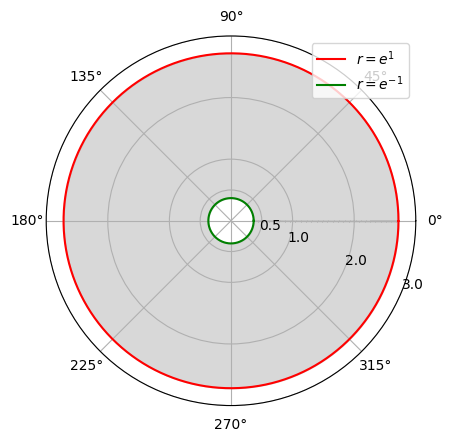
\includegraphics[width=\linewidth]{FIG_MAT215/exp z vertical strip out.png}
        \caption{$r=e^{\pm1}$}
        \label{fig:exp_outputs_h}
    \end{subfigure}
    \caption{Input and Output under the Exponential Map for Vertical Strip}
    \label{fig:exp_map_vertical_lines}
\end{figure}
Let's make things spicy! Now, we will see how the region between two vertical lines mapped in the output plane.
The vertical strip \( -1 \leq \text{Re}(z) \leq 1 \) in the \( z \)-plane maps to the annular region bounded by the circles \( r = e^{-1} \) and \( r = e^{1} \) in the \( w \)-plane under the exponential map \( w = \exp(z) \), let’s analyze how the exponential map transforms each component of \( z = x + iy \). The range of \( x \) in the vertical strip is given by \( -1 \leq x \leq 1 \).\\
When \( x = 1 \), we have:
   \[
   |w| = e^1 = e.
   \]
   So, points on the line \( x = 1 \) in the \( z \)-plane are mapped to points on the circle of radius \( r = e \) in the \( w \)-plane.\\
When \( x = -1 \), we have:
   \[
   |w| = e^{-1} = \frac{1}{e}.
   \]
   Thus, points on the line \( x = -1 \) in the \( z \)-plane are mapped to points on the circle of radius \( r = \frac{1}{e} \) in the \( w \)-plane.

Since \( x \) varies continuously from \( -1 \) to \( 1 \), \( |w| = e^x \) will take all values between \( e^{-1} \) and \( e \). Therefore, the modulus \( |w| \) in the \( w \)-plane lies in the range:
\[
e^{-1} \leq |w| \leq e.
\]
This defines an annular region bounded by the circles \( r = e^{-1} \) and \( r = e \) in the \( w \)-plane. The imaginary part \( y \) of \( z \) becomes the angle \( \arg(w) \) in the \( w \)-plane. Since \( y \) can vary freely from \( -\infty \) to \( +\infty \), \( \arg(w) \) will cover all possible angles from \( -\infty \) to \( +\infty \). This means that \( w \) wraps around the annular region \textbf{infinitely many times} as \( y \) varies, covering every point in the annulus.
\begin{exercise}
    Find the output region for the horizontal strip in $z$-plane we mentioned above (between $z=x+\frac{\pi}{4}i$ and $z=x-\frac{\pi}{4}i$). 
\end{exercise}
\subsection{Complex powers}
With the logarithm function at our disposal, we are able to define complex powers of complex numbers. Let $\alpha$ be a complex number. The for all $z \neq 0$, we define the $\alpha$-th power $z^\alpha$ of $z$ by
$$
\boxed{z^\alpha \equiv e^{\alpha \log (z)}=e^{\alpha \log |z|+i \alpha \arg (z)}}
$$
The multiple-valuedness of the argument means that generically there will be an infinite number of values for $z^\alpha$. We can rewrite the above expression a little to make this manifest:
$$
z^\alpha=e^{\alpha \log |z|+i \alpha \operatorname{Arg}(z)+i \alpha 2 \pi k}=e^{\alpha \log (z)} e^{i \alpha 2 \pi k},
$$
for $k=0, \pm 1, \pm 2, \ldots$
Depending on $\alpha$ we will have either one, finitely many or infinitely many values of $\exp (i 2 \pi \alpha k)$.
\begin{exercise}
    Find $i^i$ and $1^i$. 
\end{exercise}
\section{Complex Trigonometry! Ugh!}
Before we start talking about complex trigonometric functions, let's look at the hyperbolic functions. We already knew that, 
\begin{align*}
    \sinh{x}&=\frac{e^x-e^{-x}}{2}\\
    \cosh{x}&=\frac{e^x+e^{-x}}{2}\\
    \tanh{x}&=\frac{e^x-e^{-x}}{e^x+e^{-x}}
\end{align*}
Okay, now without worrying about anything just plug in the complex numbers (purely imaginary) in the trigonometric function! 
\begin{align*}
    \cos(ix)&=\frac{e^{i(ix)}+e^{-i(ix)}}{2}\\
    &= \frac{e^{-x}+e^{x}}{2}\\
    &= \frac{e^x+e^{-x}}{2}\\
    &= \cosh{x}
\end{align*}
In a similar fashion, we can get
\begin{align*}
    \sin{ix}&=i\sinh{x}\\
    \tan{ix}&=i\tanh{x}
\end{align*}
Nice! But we need to plug in the general complex number $(z=a+ib)$, so let's give it a try also,
\begin{align*}
    \sin(x+iy)&=\sin(x)\cos(iy)+\cos(x)\sin(iy)\\
    &= \sin(x)\cosh(y)+\cos(x)i\sinh(y)\\
    &= \sin(x)\cosh(y)+i\cos(x)\sinh(y)
\end{align*}
\textbf{Question:} Do we have the same properties (nicer) of trigonometric function in complex variables?\\
\begin{example}
    Similarly, we can show that, $$\cos{z}=\cos(x+iy)=\cos x\cos(iy)-\sin x\sin(iy)=\cos x\cosh y-i\sin x\sinh y$$
\end{example}
\begin{example}
    \textbf{Question:} Show that, $$\sin(-z)=\sin(z)$$
\end{example}
\begin{example}
    \textbf{Question:} Show that, $$\sin(z+2\pi)=\sin(z)$$
\end{example}
\begin{example}
% https://ximera.osu.edu/math/complexBook/complexBook/complexTrig/complexTrig
\textbf{Question:} Solve for $\sin (z)=2$ where $z\in\mathbb C$.\\
\textbf{Answer:} Since
$$
\sin (z)=\sin (x) \cosh (y)+i \cos (x) \sinh (y)
$$
we need
$$
\sin (x) \cosh (y)=2 \text { and } \cos (x) \sinh (y)=0
$$
simultaneously. The second equation is eeasier to work with because we can use the zero product principle. It gives:
$$
x=\pi / 2+k \pi \text { or } y=0
$$
We substitute these results into the first equation one at at time. If $y=0$, the first equation becomes:
$$
\sin (x) \cosh 0=2
$$
Since $\cosh (0)=1$, this leads to the equation $\sin (x)=2$ which has no solutions.
Next, if $x=\pi / 2+k \pi$ then $\sin (x)= \pm 1$. Thus we consider cases. If where $k$ is even, then
$$
\sin (x)=\sin \left(\frac{\pi}{2}+k \pi\right)=1
$$
and we arrive at
$$
\cosh (y)=2
$$
which has two solutions (verify)
$$
y=\ln (2 \pm \sqrt{3})
$$
Finally, if $x=\pi / 2+k \pi$ where $k$ is odd, then
$$
\sin (x)=\sin \left(\frac{\pi}{2}+k \pi\right)=-1
$$
and we arrive at
$$
\cosh (y)=-2
$$
which has no solutions (verify). Thus the equation $\sin (z)=2$ has as its solutions
$$
z=\left[\frac{\pi}{2}+k \pi\right]+i[\ln (2 \pm \sqrt{ } 3)]
$$
where $k$ is an even integer.
\end{example}

\begin{example}
\textbf{Question:} Find the image of the given line under the given map, 
    \begin{enumerate}
        \item $Im(z)=1;\quad f(z)=\cos(z)$
        \item $Re(z)=\frac{\pi}{6};\quad f(z)=\sin(z)$
    \end{enumerate}
\textbf{Answer:} (1) Using the formula for \( \cos(z) \) in terms of exponential functions:
\[
\cos(z) = \cos(x + i) = \frac{e^{i(x+i)} + e^{-i(x+i)}}{2}.
\]
Simplify \( e^{i(x+i)} \) and \( e^{-i(x+i)} \):
\[
e^{i(x+i)} = e^{-1} e^{ix}, \quad e^{-i(x+i)} = e^{-1} e^{-ix}.
\]
Thus:
\[
\cos(z) = \frac{e^{-1} e^{ix} + e^{-1} e^{-ix}}{2} = e^{-1} \frac{e^{ix} + e^{-ix}}{2}.
\]
Recognizing \( \frac{e^{ix} + e^{-ix}}{2} = \cos(x) \):
\[
\cos(z) = e^{-1} \cos(x).
\]
Since \( x \in \mathbb{R} \), \( \cos(x) \) takes values in \([-1, 1]\). Therefore: $f(z) = \cos(z)$ maps the line $\operatorname{Im}(z) = 1$ to the horizontal segment $\left[-\frac{1}{e}, \frac{1}{e}\right]$ on the real axis.\\~\\
(2) If \( \operatorname{Re}(z) = \frac{\pi}{6} \), we can write \( z = \frac{\pi}{6} + iy \), where \( y \in \mathbb{R} \).

Using the formula for \( \sin(z) \) we get:
\begin{align*}
    \sin\left(\frac{\pi}{6}+iy\right) &= \sin\left(\frac{\pi}{6}\right)\cosh(y)+i\cos\left(\frac{\pi}{6}\right)\sinh(y)\\
                &= \underbrace{\frac{1}{2} \cosh(y)}_u + i \underbrace{\frac{\sqrt{3}}{2} \sinh(y)}_v    
\end{align*}
Now, we want a relation between $u$ and $v$ in order to get equation for $w$-plane. We knew that,
\[
\cosh^2(y) - \sinh^2(y) = 1.
\]
Substitute the expressions for \( u \) and \( v \):
\[
\left(2 u\right)^2 - \left(\frac{2}{\sqrt{3}} v\right)^2 = 1.
\]
The relationship between \( u \) and \( v \) is a hyperbola.
This shows that the image of the line \( \operatorname{Re}(z) = \frac{\pi}{6} \) under \( f(z) = \sin(z) \) is a branch of a hyperbola in the \( w \)-plane.
\end{example}


\chapter{Limit}
\begin{example}
    \textbf{Question:} Find $$\lim_{z\rightarrow e^{\pi i/3}}(z-e^{\pi i/3})\frac{z}{z^3+1}$$
    \textbf{Answer:} We knew that, $e^{i\pi}=-1$ which implies $z^3+1=e^{i\pi}+1=-1+1=0$. That means direct substitution will produce $\frac{0}{0}$. So, we can apply L'Hopital rules here. 
    \begin{align*}
    \lim_{z \to e^{\pi i/3}} (z - e^{\pi i/3}) \frac{z}{z^3 + 1} 
    &= \lim_{z \to e^{\pi i/3}} \frac{z^2 - e^{\pi i/3} z}{z^3 + 1} \\
    &= \lim_{z \to e^{\pi i/3}} \frac{(2z - e^{\pi i/3})}
    {3z^2}\\
    &= \frac{e^{\pi i/3}}{3e^{2\pi i/3}}\\
    &= \frac{1}{3}e^{-\pi i/3}
\end{align*}
\end{example}
\begin{example}
    \textbf{Question:} Find $$\lim_{z\rightarrow0}\left(\frac{\sin z}{z}\right)^{\frac{1}{z^2}}$$
    \textbf{Answer:} Let 
    \begin{align*}
        w&=\lim_{z\rightarrow0}\left(\frac{\sin z}{z}\right)^{\frac{1}{z^2}}\\
        \ln w&= \ln\left[ \lim_{z\rightarrow0}\left(\frac{\sin z}{z}\right)^{\frac{1}{z^2}}\right]\\
        &= \lim_{z\rightarrow0}\left[ \ln\left(\frac{\sin z}{z}\right)^{\frac{1}{z^2}}\right]\\
        &=\lim_{z\rightarrow0} \frac{1}{z^2}\ln\left(\frac{\sin z}{z}\right)\\
        &= \lim_{z\rightarrow0} \frac{\ln\left(\frac{\sin z}{z}\right)}{z^2}\\
        &=\lim_{z\rightarrow0} \frac{\ln(\sin z)-\ln z}{z^2}\\
        &\stackrel{\operatorname{LH}}{=} \lim_{z\rightarrow0} \frac{\frac{1}{\sin z}\cos z-\frac{1}{z}}{2z}\\
        &=\lim_{z\rightarrow0} \frac{z\cos z-\sin z}{2z^2\sin z}
    \end{align*}
    \begin{align*}
       \ln w &\stackrel{\operatorname{LH}}{=} \lim_{z\rightarrow0} \frac{\cos z+z\cdot (-\sin z)-\cos z}{4z\sin z+2z^2\cos z}\\
        &=\lim_{z\rightarrow0} \frac{-z\sin z}{4z\sin z+2z^2\cos z}\\
        &\stackrel{\operatorname{LH}}{=} \lim_{z\rightarrow0} \frac{-\sin z -z\cos z}{4\sin z+8z\cos z-2z^2\sin z}\\
        &\stackrel{\operatorname{LH}}{=}\lim_{z\rightarrow0} \frac{-\cos z-\cos z-z(-z\sin z)}{\cdots}\\
        &= \frac{-1-1}{4+8}\\
        &= -\frac{1}{6}
    \end{align*}
\end{example}
\begin{example}
    Show that the limit does not exist, 
    $$\lim_{z\rightarrow0}\frac{\bar z}{z}$$
\end{example}

\begin{example}
    Show that the limit does not exist, 
    $$\lim_{z\rightarrow0}\frac{xy}{x^2+y^2}$$
\end{example}
\begin{example}
    \textbf{Question:} Find all the discontinuous points for $f(z)=\cot(z)$.\\
    \textbf{Answer:} 
    \begin{align*}
        f(z)&=\cot(z)\\
        &= \frac{\cos z}{\sin z}
    \end{align*}
    Discontinuous at $\sin z=0$ which implies, 
    \begin{align*}
        \frac{e^{iz}-e^{-iz}}{2i}&=0\\
        e^{iz}&=e^{-iz}\\
        \frac{e^{iz}}{e^{-iz}}&=1\\
        e^{2iz}&=1\\
        e^{2iz}&=e^{i(0+2\pi k)}\\
        2z&= 2\pi k\\
        z &= k\pi,k\in\mathbb Z 
    \end{align*}
\end{example}







\section{Exercise}
\begin{exercise}
Let $f(z)=\begin{cases}
    \frac{z^2+4}{z-2i},z\neq 2i\\
    3+4i,z=2i
\end{cases}$. Is $f(z)$ continuous at $z=2i$?
\end{exercise}
\begin{exercise}
    Find all points of discontinuity for the function, $$f(z)=\frac{2z-3}{z^2+2z+2}$$
\end{exercise}
\begin{exercise}
    Find the following limits,
$$\lim_{z\rightarrow0}\frac{z-\sin(z)}{z^3}, \lim_{z\rightarrow0}\frac{\tan(z)-\sin(z)}{z^3}$$
\end{exercise}
\begin{exercise}
    If $f(z)=\begin{cases}
        \frac{z^2-4}{z^2-3z+2},z\neq 2\\
        kz^2+6,z=2
    \end{cases}$, find $k$ such that the function $f(z)$ becomes continuous at $z=2$. 
\end{exercise}


\chapter{Differentiation}
$\mathcal N(x)$ will denote the neighborhood at point $x$. 
\begin{defn}[Geometric]
The derivative is the slope of a line tangent to the graph of the
function, if the graph has a tangent.
\end{defn}

\begin{defn}[Approximation]
The derivative of a function is the best linear approximation to the function near a point.
\end{defn}

\begin{defn}[Infinitesimal]
The ratio of the infinitesimal change in the value of a function to the infinitesimal change in a function.
\end{defn}
If we start out with $f:\mathbb{R}\to\mathbb{R}$, then $f'(c)$ is an approximation of how $f$ changes in a small interval around $x=c$.  For example, let $f(x)=x^2$, and $c=2$.  Then $f'(2)=4$.  Notice that $f(1.01)=1.0201$.  Then the change from $f(1)$ to $f(1.01)$ is $0.0201$.  This is approximately $2(.01)=0.02$.  
\\~\\
\textbf{For higher dimensions}, the derivative needs to be a transformation between $\mathbb{R}^n$ and $\mathbb{R}^m$.  For example, take $f(x,y)=(x^2,y^2)$.  Then the derivative is
$$
J_{ij}=\frac{\partial f_i}{\partial x_j}=\begin{pmatrix}
    \nabla^T f_1\\\nabla^T f_2
\end{pmatrix}=\begin{pmatrix}
2x & 0 \\ 0 & 2y
\end{pmatrix}.
$$
At $(x,y)=(1,1)$ this is
$$
\begin{pmatrix}
2 & 0 \\ 0 & 2
\end{pmatrix}.
$$
Moving from $f(1,1)=(1,1)$ to $f(1.01,1.01)=(1.0201,1.0201)$. The change between the function values is $(0.0201,0.0201)$.  Notice that
$$
\begin{pmatrix}
2 & 0 \\ 0 & 2
\end{pmatrix}
\begin{pmatrix}
0.01 \\ 0.01
\end{pmatrix}
=
\begin{pmatrix}
0.02 \\ 0.02
\end{pmatrix}.
$$
Again, very close.  So, the derivative is the linear transformation that most closely fits the function.  Since linear transformations are much easier to study than functions in general, we may learn a lot about the function from its derivatives.
\\~\\
One approach is to use the fact the "differentiability" is equivalent to "approximate linearity", in the sense that if $f$ is defined in some neighborhood of $a$, then
$$
f'(a) = \lim_{h \to 0} \frac{f(a + h) - f(a)}{h}\quad\text{exists}
$$
if and only if
$$
f(a + h) = f(a) + f'(a) h + o(h)\quad\text{at $a$ (i.e., "for small $h$").}
$$
Before delving deeply into the complex realm, let's grasp the most essential tool for comprehending a complex plane (complex vector space, complex manifold): the holomorphic function. A common query might arise: If we consider points in the complex plane akin to vectors in \(\mathbb{R}^2\), does differentiability in \(\mathbb{R}^2\) extend to the complex plane as well? The answer is no; complex differentiability is significantly more constrained. For if a function $f:\mathbb R^2\rightarrow\mathbb R^2$ is differentiable at a point $x\in\mathbb R^2$ we can locally approximate it by a linear map that's why we have,
$$f(x+h)=f(x)+Ah+o(h),\qquad h\rightarrow0$$
where $A:\mathbb R^2\rightarrow\mathbb R^2$ is a linear transformation. Now we can do the same thing for a complex linear map,
$$f(x+h)=f(x)+\Tilde a\cdot h+o(h),\qquad h\rightarrow0$$
where $\Tilde a\in\mathbb C$. Then we can see the complex multiplication $\Tilde a\cdot h$ as a complex linear map which can be represented by a matrix form because we consider $\Tilde{a}$ as a mapping $\mathbb{R}^2\rightarrow\mathbb{R}^2$,

$$
\underbrace{\begin{pmatrix}
    \Re \Tilde a & -\Im \Tilde a\\ \Im \Tilde a & \Re \Tilde a
\end{pmatrix}}_{\Tilde{a}}
\underbrace{\begin{pmatrix}
    \Re h\\ \Im h
\end{pmatrix}}_{h}=
\begin{pmatrix}
    \Re \Tilde a \Re h & -\Im \Tilde a\Im h\\ \Im \Tilde a \Re h & \Re \Tilde a\Im h
\end{pmatrix}
$$
This encodes the complex multiplication $\Tilde a\cdot h=(\Re \Tilde a +\Im \Tilde a)\cdot (\Re h +\Im h)=(\Re \Tilde a \Re h -\Im \Tilde a\Im h)+i(\Im \Tilde a \Re h + \Re \Tilde a\Im h)$, but not all linear maps which arise from $\mathbb R$-differentiable function look like this.\\~\\
A function $f(z)$ is said to be analytic or holomorphic at $z_0$ if one of the following equivalent conditions holds:
\begin{enumerate}[label=\textbf{C\arabic*}]
    \item \label{hol_C_1} We can consider $f$ as a function of two real variables $f(x,y)$. And we can decompose it as $f(x,y)=u(x,y)+iv(x,y)$, where $u(x,y)$ and $v(x,y)$ denote the real and imaginary part of $f$ respectively. Then we want the first partial derivatives to exist and be continuous and further satisfy the CR equations, $$u_x=v_y,\quad v_x=-u_y$$
    \item \label{hol_C_2} The limit exists $$\lim_{\Delta  z\rightarrow0}\frac{f(z+\Delta z)-f(z)}{\Delta z}\quad\forall z\in \mathcal N(z_0)$$
    \item \label{hol_C_3} $\exists$ a power series of the form $\sum a_n (z-z_0)^n$ which is convergent to $f(z)$ for each point $z$ in a neighborhood of $z_0$.
\end{enumerate}


\begin{example}
    \textbf{Question:} Show that $f(z)=\operatorname{Re}(z)$ is nowhere differentiable.\\
    \textbf{Answer:} We know that a function is differentiable at point $z_0$ if the following limit exists, $$\lim_{h\rightarrow0}\frac{f(z_0+h)-f(z_0)}{h}$$
    Remember, both $z_0$ and $h$ are complex numbers. Let's choose an arbitrary point $z\in\mathbb{C}$ and substitute $z=x+iy$ and $h=h_x+ih_y$ then, 
    \begin{align*}
        \frac{f(z+h)-f(z)}{h}&=\frac{\operatorname{Re}(z+h)-\operatorname{Re}(z)}{h}\\
        &= \frac{\operatorname{Re}(x+iy+h_x+iy)-\operatorname{Re}(x+iy)}{h}\\
        &= \frac{\operatorname{Re}((x+h_x)+i(y+h_y))-\operatorname{Re}(x+iy)}{h}\\
        &= \frac{x+h_x-x}{h}\\
        &= \frac{h_x}{h}
    \end{align*}
    Now, we will consider different different paths and show they give different different values.\\ 
    \textbf{Path 1 - Along the real axis}\\
    If we approach the origin along the real axis then we have, $h=h_x+i\cdot 0$ which implies $\operatorname{Re}(h)=h_x\equiv h=h_x+i\cdot0$. Hence, 
    \begin{align*}
        \lim_{h\rightarrow0} \frac{h_x}{h}&= \lim_{h_x\rightarrow0} \frac{h_x}{h_x+i\cdot0}\\
        &= \lim_{h_x\rightarrow0} \frac{h_x}{h_x}\\
        &= \lim_{h_x\rightarrow0} 1\\
        &= 1
    \end{align*}
    \textbf{Path 1 - Along the imaginary axis}\\
    If we approach the origin along the imaginary axis then we have, $h=0+i\cdot h_y$ which implies $\operatorname{Re}(h)=0$. Hence,
    \begin{align*}
        \lim_{h\rightarrow0} \frac{h_x}{h}&= \lim_{h_y\rightarrow0} \frac{h_x}{0+ih_y}\\
        &= \lim_{h_y\rightarrow0} \frac{0}{ih_y}\\
        &= 0
    \end{align*}
    Voila! We show that the limit doesn't exist when we choose two different paths for which $h\rightarrow0$.\\~\\ 
    \textbf{Alternative:} While choosing different paths to solve this kind of limit problem, getting the same values for two paths might be very problematic. Hence, we can solve this problem by choosing a special path. Like $h_n=\frac{i^n}{n}$ shown in figure \ref{fig:Re_z_diff}. Now, we have
    \begin{align*}
        \lim_{h_n\rightarrow0} \frac{\operatorname{Re}(h_n)}{h_n} &= \lim_{h_n\rightarrow0} \frac{\frac{\operatorname{Re}(i^n)}{n}}{\frac{i^n}{n}}\\
        &= \begin{cases}
            1,n\text{ is even}\\
            0,n\text{ is odd}
        \end{cases}
    \end{align*}
    The end result depends on the value of $n$. Hence, the limit doesn't exist. 
\end{example}
\begin{figure}
        \centering
        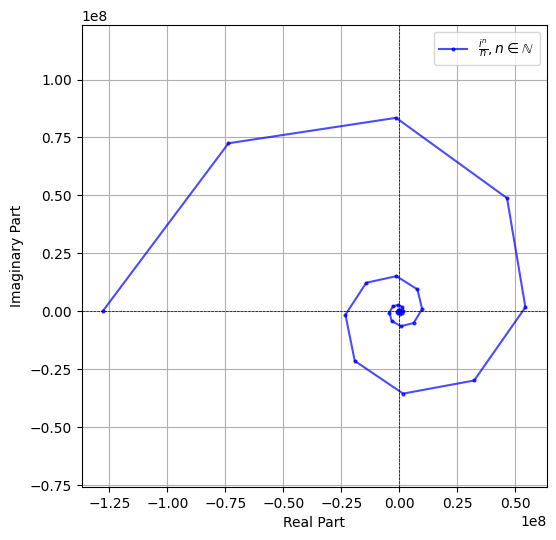
\includegraphics[width=0.5\linewidth]{FIG_MAT215/Re_z.png}
        \caption{$\frac{i^n}{n}$}
        \label{fig:Re_z_diff}
    \end{figure}
\begin{example}
\textbf{Question:} Prove that $f(z) = |z|^2$ is differentiable only at the origin.\\
\textbf{Answer:} 
Pick any arbitrary point $z_0 \in\mathbb C$. Then check the differentiability at that point. Besides, we knew that, $|z|^2=z\bar z$. 
\begin{align*}
    \lim_{\Delta z\rightarrow0}\frac{f(z_0+\Delta z)-f(z_0)}{\Delta z}&= \lim_{\Delta z\rightarrow0} \frac{\mid z_0+\Delta z\mid^2 - |z_0|^2}{\Delta z}\\
    &= \lim_{\Delta z\rightarrow0} \frac{(z_0+\Delta z)(\overline{z_0+\Delta z})-z_0\overline{z_0}}{\Delta z}\\
    &= \lim_{\Delta z\rightarrow0} \frac{z_0\overline{z_0}+z_0\overline{\Delta z}+\Delta z\overline{z_0}+\Delta z\overline{\Delta z}-z_0\overline{z_0}}{\Delta z}\\
    &= \lim_{\Delta z\rightarrow0} z_0\frac{\overline{\Delta z}}{\Delta z}+\overline{z_0}+\overline{\Delta z}
\end{align*}
Here, we can't substitute $\Delta z=0$ in the expression. Hence, to find the limit value we need to consider pathwise value.\\ 
\textbf{Path-I: Consider the $x$-direction:}\\
Here, $y=0$ hence $\Delta y=0$. And we know that, $\Delta z=\Delta x+i\Delta y=\Delta x$. Even $\overline{\Delta z}=\Delta x - i\Delta y=\Delta x$. And $\Delta z\rightarrow 0 \implies \Delta x\rightarrow 0$. Now, using all these information rewrite the limit expression:
\begin{align*}
    \lim_{\Delta z\rightarrow0} z_0\frac{\overline{\Delta z}}{\Delta z}+\overline{z_0}+\overline{\Delta z} &= \lim_{\Delta x\rightarrow 0} z_0 \frac{\Delta x}{\Delta x} + \overline{z_0} + \Delta x\\
    &= \lim_{\Delta x\rightarrow 0} z_0 + \overline{z_0} +\Delta x\\
    &= \boxed{z_0\cdot 1 + \overline{z_0} + 0}
\end{align*}
Similarly, For \textbf{Path-II: Consider the $y$-direction:}\\
Here, $x=0$ hence $\Delta x=0$. And we know that, $\Delta z=\Delta x+i\Delta y=i\Delta y$. Even $\overline{\Delta z}=\Delta x- i\Delta y=-i \Delta y$. And $\Delta z\rightarrow 0 \implies \Delta y\rightarrow 0$. Now, using all these information rewrite the limit expression:
\begin{align*}
    \lim_{\Delta z\rightarrow0} z_0\frac{\overline{\Delta z}}{\Delta z}+\overline{z_0}+\overline{\Delta z} &= \lim_{\Delta y\rightarrow 0} z_0 \frac{i \Delta y}{-i \Delta y} + \overline{z_0} + \Delta y\\
    &= \lim_{\Delta y\rightarrow 0} z_0\cdot -1 + \overline{z_0} +\Delta y\\
    &= \boxed{-z_0 + \overline{z_0} + 0}
\end{align*}
Equating the limit values we get:
\begin{align*}
    z_0+\overline{z_0} &= z_0 + \overline{z_0}\\
    2z_0 &= 0\\
    z_0 &= 0
\end{align*}
Which mean the function is only differentiable at point $z=0$. Except that point the function is not differentiable. 
% $f$ is differentiable at $0$ is simply to observe that$$\lim_{z\to0}\frac{|z|^2}z=\lim_{z\to0}\overline z=0.$$Besides, if $z_0\neq0$, then$$\lim_{z\to z_0}\frac{|z|^2-|z_0|^2}{z-z_0}=\lim_{z\to z_0}\frac{|z|-|z_0|}{z-z_0}\bigl(|z|+|z_0|\bigr).$$
% To see why it does not exist by taking two different paths of approach to \( z_0 \). The two paths we will use are:
% \begin{enumerate}
%     \item Along a circle centered at \( 0 \) and passing through \( z_0 \)
%     \item Along a ray from \( 0 \) passing through \( z_0 \) 
% \end{enumerate}
% \textbf{Path 1 – Approaching \( z_0 \) along a Circle Centered at \( 0 \)}\\
% If \( z \) is on the same circle as \( z_0 \) (centered at \( 0 \)), then \( |z| = |z_0| \). This means that:
% \[
% |z|^2 - |z_0|^2 = 0.
% \]
% Thus, along this path, we have:
% \[
% \frac{|z|^2 - |z_0|^2}{z - z_0} = \frac{0}{z - z_0} = 0.
% \]
% So, along this circular path, the limit is \( 0 \).\\~\\
% \textbf{Path 2 – Approaching \( z_0 \) along a Ray from \( 0 \)}\\
% Now consider the path where \( z \) approaches \( z_0 \) along the ray starting from \( 0 \). We can parameterize this path by setting \( z = \lambda z_0 \) with \( \lambda \in (1, +\infty) \), so \( \lambda \to 1 \) as \( z \to z_0 \).

% In this case:
% - \( |z| = |\lambda z_0| = \lambda |z_0| \),
% - \( |z|^2 = \lambda^2 |z_0|^2 \),
% - and \( z - z_0 = \lambda z_0 - z_0 = (\lambda - 1) z_0 \).

% Now let’s compute the limit:
% \[
% \frac{|z|^2 - |z_0|^2}{z - z_0} = \frac{\lambda^2 |z_0|^2 - |z_0|^2}{(\lambda - 1) z_0}.
% \]
% Factor \( |z_0|^2 \) from the numerator:
% \[
% = \frac{|z_0|^2 (\lambda^2 - 1)}{(\lambda - 1) z_0}.
% \]
% Now factor \((\lambda - 1)\) from \( \lambda^2 - 1 = (\lambda - 1)(\lambda + 1) \):
% \[
% = \frac{|z_0|^2 (\lambda - 1)(\lambda + 1)}{(\lambda - 1) z_0} = \frac{|z_0|^2 (\lambda + 1)}{z_0}.
% \]
% Now cancel \( |z_0| \) from \( |z_0|^2 \) with one \( z_0 \) in the denominator, and you get:
% \[
% = \overline{z_0} \cdot (\lambda + 1).
% \]
% Taking the limit as \( \lambda \to 1 \):
% \[
% \lim_{\lambda \to 1} \overline{z_0} (\lambda + 1) = \overline{z_0} \cdot 2 = 2 \overline{z_0}.
% \]
% So, along this ray, the limit is \( 2 \overline{z_0} \neq 0 \).


% Now, if $z$ approaches $z_0$ along the circle centered at $0$ passing through $z_0$, then the previous limit is $0$. And if $z$ approaches $z_0$ along the ray $\bigl\{\lambda z_0\,|\,\lambda\in(1,+\infty)\bigr\}$, then the previous limit is $2\overline{z_0}\neq0$. Therefore the limit does not exist.
\end{example}

\begin{example}
\textbf{Question:} Determine a harmonic conjugate to the function \begin{equation*} f(x,y)=2y^{3}-6x^{2}y+4x^{2}-7xy-4y^{2}+3x+4y-4 \end{equation*}

We first of all check if $f(x,y)$ is indeed a harmonic function. This amounts to show $f(x,y)$ satisfy the two-dimensional Laplace equation
\begin{equation*}
\frac{\partial^{2 }f}{\partial x^{2}}+\frac{\partial^{2} f}{\partial y^{2}}=0 \tag{1}
\end{equation*}
We have $\frac{\partial^{2}f}{\partial x^{2}}=8-12y$ and $\frac{\partial^{2} f}{\partial y^{2}}=12y-8$. Thus, (1) is fulfilled, and so $f(x,y)$ is harmonic. 

Next, we seek to determine a harmonic conjugate to the given function. Let $u(x,y)=2y^{3}-6x^{2}y+4x^{2}-7xy-4y^{2}+3x+4y-4$. 
\begin{equation*}
u_{x}=v_{y} \iff -12xy+8x-7y+3=v_{y}
\end{equation*}
Integrate with respect to $y$
\begin{equation*}
v=-6xy^{2}+8xy-\frac{7}{2}y^{2}+3y+h(x) \tag{2}
\end{equation*}
where $h(x)$ is a function of $x$ alone. To determine this, we use the second Cauchy-Riemann equation* $v_{x}=-u_{y}$ 
\begin{align*}
-u_{y}=v_{x} &\iff 6x^{2}+7x-6y^{2}+8y-4=h'(x)-6y^{2}+8y \\
&\iff h'(x)=6x^{2}+7x-4
\end{align*}
Integrating with respect to $x$ we have
\begin{equation*}
h(x)=2x^{3}+\frac{7}{2}x^{2}-4x+C
\end{equation*}
where $C$ is an arbitrary constant. Therefore, if we let $C=0$, then one harmonic conjugate of $u$ is given as:
\begin{equation*}
v=2x^{3}+\frac{7}{2}x^{2}-6xy^{2}+8xy-4x-\frac{7}{2}y^{2}+3y
\end{equation*}
\textbf{Yet another shortcut.} Since $u$ is harmonic (on the simply connected domain $\mathbb{C}$), there has to be a harmonic conjugate $v$. Let $F = u+iv$ be the corresponding holomorphic function. It follows from (the derivation of) Cauchy Riemann's equations that:
$$
F' = u'_x - i\,u'_y = -12xy + 8x -7y + 3 + i(6x^2+7x-6y^2+8y-4).
$$
Let $G(z) = 3 +  8z + i(6z^2+7z-4)$. Then $G(z) = F'(z)$ if $z$ is real, so by the identity theorem, $G = F'$ for all $z$. Hence
$$
F(z) = 3z + 4z^2 - 4 + i(2z^3+\frac72z^2-4z+C)
$$
for some real constant $C$ (the real part of the constant of integration has to be $4$ to match $u$). Finally
$$
v = \operatorname{Im}(F(z)).
$$
\end{example}

\chapter{Line Integral}
\begin{itemize}
    \item If you can easily parameterize your curve $C$ by $\gamma(t)$ then use: 
    $$\int_Cf(z)dz\stackrel{C=\gamma(t)}{=\joinrel=}\int_\gamma f(\gamma(t))\gamma'(t)dt$$
    For example, if our curve is a circle $|z-z_0|=R$ then we can parametrize it by $\gamma(t)=z_0+Re^{it},0\geq t\geq 2\pi$.     
    \item If you can deform your parametrization from initial path $\gamma_1(t)$ to final path $\gamma_2(t)$ without hitting any singularities then:
    $$\int_{\gamma_1}f(z)dz=\int_{\gamma_2}f(z)dz$$
\end{itemize}
\begin{figure}[h]
    \centering
    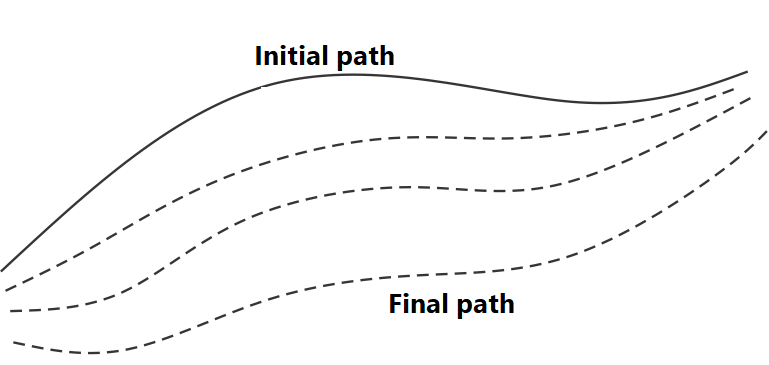
\includegraphics[width=0.4\textwidth]{FIG_MAT215/path deform.png}
    \caption{Path deformation: while deforming the initial path, we didn't hit any singularities}
    \label{fig:path_deform}
\end{figure}
\begin{itemize}
    \item (\textbf{Cauchy's theorem}) If the curve is closed and our function $f(z)$ is analytic on the region $D$ enclosed by the curve then, 
    $$\int_\gamma f(z)dz=0$$
    \item (\textbf{Cauchy's integral formula}) Suppose $C$ is a simple closed curve and the function $f(z)$ is analytic on the region $D$ closed by the curve. We assume $C$ is oriented counterclockwise. Then for any $z_0$ inside $C$: $$f(z_0)=\frac{1}{2\pi i}\int_C \frac{f(z)}{z-z_0}dz$$
\end{itemize}
\begin{figure}[h]
    \centering
    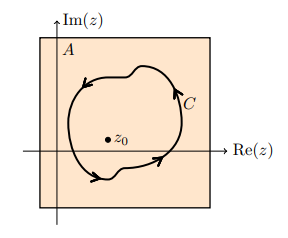
\includegraphics[width=0.4\textwidth]{FIG_MAT215/cauchy_formula_temp.PNG}
    \caption{Cauchy integral formula}
    \label{fig:CIF}
\end{figure}
\begin{itemize}
    \item (\textbf{Cauchy's integral formula for derivatives}) If $f(z)$ and $C$ satisfy the same hypotheses as for Cauchy's integral formula then, for all $z_0$ inside $C$ we have: $$f^{(n)}(z_0)=\frac{n!}{2\pi i}\int_C \frac{f(z)}{(z-z_0)^{n+1}}dz$$
    \item (\textbf{Cauchy's residue theorem}) Suppose $f(z)$ is analytic in the region $A$ except for a set of isolated singularities. Also, suppose $C$ is a simple closed curve in $A$ that doesn't go through any of the singularities of $f$ and is oriented counterclockwise. Then $$\int_C f(z) d z=2 \pi i \sum \text{ residues of } f \text { inside } C$$
    To calculate residue at the pole $z_0$ with degree $k$, we use:
    $$\operatorname{Res}(f,z_0)=\lim_{z\rightarrow z_0}\frac{1}{(k-1)!}\frac{d^{k-1}}{dz^{k-1}}\left[(z-z_0)^k f(z)\right]$$
    But we can compute it easily using a series in our function if possible.  
\end{itemize}

\chapter{Laplace Transformation}
\section{Derivation}
We knew that, 
\begin{align*}
    F(s)&=\int_0^\infty f(t) e^{-st}dt\\
    \frac{d}{ds} F(s) &= \frac{d}{ds} \int_0^\infty f(t) e^{-st}dt\\
    &\stackrel{\text{Leibnitz}}{=} \int_0^\infty f(t) \frac{\partial}{\partial s} e^{-st} dt\qquad \text{(also use Dominated convergence theorem)}\\
    &= - \int_0^\infty  tf(t) e^{-st} dt\\
    -\frac{d}{ds} F(s) &= \mathcal{L}\{tf(t)\}\qed 
\end{align*}
Again, we use Fubini's theorem to derive the integral formula, 
$$\int_s^\infty F(s)=\int_0^\infty f(t)\left(\int_s^\infty e^{-ut}du\right)dt$$
We can categorize all the examples into $ 6$ types. 
\begin{enumerate}
    \item Known formula 
    \item $$\mathcal L\{e^{at}f(t)\}=\mathcal L\{f(t)\}_{s\rightarrow s-a}=F(s-a)$$
    $$\underbrace{\mathcal L^{-1}\{F(s)\}}_{\text{unknown}}=e^{at}\underbrace{\mathcal L^{-1}\{F(s+a)\}}_{\text{known}}$$
    \item $$\mathcal{L}\{f(t)u(t-a)\}=\mathcal{L}\{f(t+a)\}e^{-as}$$
    $$\mathcal{L}^{-1}\{F(s)e^{-as}\}=f(t-a)u(t-a)$$
    \item Partial fraction type
    \item $s$-differentiation 
    \item Convolution type
\end{enumerate}

\section{Type-5}

\textbf{Question:} Find the inverse Laplace Transformation of $\frac{2s}{(s^2+1)^2}$.\\
\textbf{Answer:} Use the formula, $$\mathcal{L}\{t f(t)\}=-\frac{d}{ds}\mathcal{L}\{f(t)\}$$
We already know that, $$\mathcal{L}\{\sin (t)\}=\frac{1}{s^2+1}$$
Then, 
\begin{align*}
    \mathcal{L}\{t\sin{t}\}&= -\frac{d}{ds}\left( \frac{1}{s^2+1} \right)\\
    &= \frac{2s}{(s^2+1)^2}
\end{align*}
\section{Type-6}
\textbf{Question:} Find the Laplace Transformation of $\frac{1}{s^2}\frac{1}{s^+1}$.\\ 
\textbf{Answer:} We already knew that, $$\mathcal{L}\left\{\frac{1}{s^2}\right\}= t\:u(t), \qquad\mathcal{L}\left\{\frac{1}{s^2+1}\right\}=\sin{t}\: u(t)$$
Now, use the convolution formula, 
\begin{align*}
    \mathcal{L}^{-1}\left\{\frac{1}{s^2}\frac{1}{s^2+1}\right\}&= \int_{-\infty}^\infty f(t-\tau)g(\tau)d\tau\\
    &= \int_{-\infty}^\infty (t-\tau)\: u(t-\tau) \sin(\tau)\: u(\tau) d\tau\\
    &\stackrel{A}{=} \int_0^t (t-\tau) \sin{\tau} d\tau 
\end{align*}
See the footnote for A\footnote{$u(t-\tau)$ force $t-\tau\geq 0\implies t\geq \tau$ and $u(\tau)$ force $\tau\geq 0$. Hence, $0\leq\tau\leq t$}. 